\documentclass[namedreferences]{solarphysics}

\usepackage[hyperref,optionalrh]{spr-sola-addons} % For Solar Physics 
%\usepackage[optionalrh]{spr-sola-addons} % For Solar Physics 
%\usepackage{epsfig}          % For eps figures, old commands
\usepackage{graphicx}        % For eps figures, newer & more powerfull
%\usepackage{courier}         % Change the \texttt command to courier style
%\usepackage{amssymb}        % useful mathematical symbols
\usepackage{color}           % For color text: \color command
\usepackage{breakurl}        % For breaking URLs easily trough lines
\def\UrlFont{\sf}            % define the fonts for the URLs

% General definitions
% please place your own definitions here and don't use \def but
% \newcommand{}{} or 
% \renewcommand{}{} if it is already defined in LaTeX

\newcommand{\BibTeX}{\textsc{Bib}\TeX}
\newcommand{\etal}{{\it et al.}}

% Definitions for equations
\renewcommand{\vec}[1]{{\mathbfit #1}}
\newcommand{\deriv}[2]{\frac{{\mathrm d} #1}{{\mathrm d} #2}}
\newcommand{\rmd}{ {\ \mathrm d} }
\newcommand{\uvec}[1]{ \hat{\mathbf #1} }
\newcommand{\pder}[2]{ \f{\partial #1}{\partial #2} }
\newcommand{\grad}{ {\bf \nabla } }
\newcommand{\curl}{ {\bf \nabla} \times}
\newcommand{\vol}{ {\mathcal V} }
\newcommand{\bndry}{ {\mathcal S} }
\newcommand{\dv}{~{\mathrm d}^3 x}
\newcommand{\da}{~{\mathrm d}^2 x}
\newcommand{\dl}{~{\mathrm d} l}
\newcommand{\dt}{~{\mathrm d}t}
\newcommand{\intv}{\int_{\vol}^{}}
\newcommand{\inta}{\int_{\bndry}^{}}
\newcommand{\avec}{ \vec A}
\newcommand{\ap}{ \vec A_p}

\newcommand{\bb}{\vec B}
\newcommand{\jj}{ \vec j}
\newcommand{\rr}{ \vec r}
\newcommand{\xx}{ \vec x}

% Definitions for the journal names
\newcommand{\adv}{    {\it Adv. Space Res.}} 
\newcommand{\annG}{   {\it Ann. Geophys.}} 
\newcommand{\aap}{    {\it Astron. Astrophys.}}
\newcommand{\aaps}{   {\it Astron. Astrophys. Suppl.}}
\newcommand{\aapr}{   {\it Astron. Astrophys. Rev.}}
\newcommand{\ag}{     {\it Ann. Geophys.}}
\newcommand{\aj}{     {\it Astron. J.}} 
\newcommand{\apj}{    {\it Astrophys. J.}}
\newcommand{\apjl}{   {\it Astrophys. J. Lett.}}
\newcommand{\apss}{   {\it Astrophys. Space Sci.}} 
\newcommand{\cjaa}{   {\it Chin. J. Astron. Astrophys.}} 
\newcommand{\gafd}{   {\it Geophys. Astrophys. Fluid Dyn.}}
\newcommand{\grl}{    {\it Geophys. Res. Lett.}}
\newcommand{\ijga}{   {\it Int. J. Geomagn. Aeron.}}
\newcommand{\jastp}{  {\it J. Atmos. Solar-Terr. Phys.}} 
\newcommand{\jgr}{    {\it J. Geophys. Res.}}
\newcommand{\mnras}{  {\it Mon. Not. Roy. Astron. Soc.}}
\newcommand{\nat}{    {\it Nature}}
\newcommand{\pasp}{   {\it Pub. Astron. Soc. Pac.}}
\newcommand{\pasj}{   {\it Pub. Astron. Soc. Japan}}
\newcommand{\pre}{    {\it Phys. Rev. E}}
\newcommand{\solphys}{{\it Solar Phys.}}
\newcommand{\sovast}{ {\it Soviet  Astron.}} 
\newcommand{\ssr}{    {\it Space Sci. Rev.}} 
\chardef\us=`\_

%%%%%%%%%%%%%%%%%%%%%%%%%%%%%%%%%%%%%%%%%%%%%%%%%%%%%%%%%%%%%%%%%%
\begin{document}

\begin{article}
\begin{opening}

\title{Article preparation guidelines\\ {\it Solar Physics}}

\author[addressref={aff1,aff2,aff3},corref,email={e-mail.a@mail.com}]{\inits{F.N.}\fnm{F. Name}~\lnm{Author-a}}%\sep
\author[addressref=aff1,email={e-mail.b@mail.com}]{\inits{F.}\fnm{Fisrt}~\lnm{Author-b}}%\sep
\author[corref,email={e-mail.c@mail.com}]{\inits{S.}\fnm{Second}~\lnm{Author-c}}%\sep
\author{\inits{T.}\fnm{Third}~\lnm{Author-x}}
%\author{\inits{}\fnm{}~\lnm{}\orcid{}}
%\author{P.~\surname{Author-a}$^{1}$\sep
%        E.~\surname{Author-b}$^{1}$\sep
%        M.~\surname{Author-c}$^{2}$      
%       }

%   \institute{$^{1}$ First affiliation
%                     email: \url{e.mail-a} email: \url{e.mail-b}\\ 
%              $^{2}$ Second affiliation
%                     email: \url{e.mail-c} \\
%             }
\address[id=aff1]{First very very very very very very very very very
 very very very very very very very very very very very very very very very very very very long affiliation}
\address[id=aff2]{Second affiliation}
\address[id=aff3]{Third affiliation}

\runningauthor{Author-a et al.}
\runningtitle{Example paper}

\begin{abstract}
0- Title / Abstract

1- Introduction. Aquí se da contexto, se anuncian las técnicas y los targets.

2- Methodology
   2.1 DEMT reconstructions.
   2.2 AWSoM simulations.
   2.3 Tracing results along fieldlines.

3- Results
   3.1 Tomographic Results. Aquí se analizan los resultados DEMT per se y también trazados a lo largo de las lineas. Se comparan las dos rotaciones entre si e incluso con tu paper previo.
   3.2 Tomography and Models

4- Discussion

Con respecto a que mostrar en la sección 3.1. Hay varias cosas. Una que Fede propone es repetir quizá de arranque la misma Figura de Rona a una altura dada versus latitudes. Eso exige saber la latitud promedio de la frontera O/C. A discutir, debo mirar el paper de Rona.
Fede, te parece que lo de arriba luce bien? Otra idea?

\end{abstract}
\keywords{Flares, Dynamics; Helicity, Magnetic; Magnetic fields, Corona}
\end{opening}
%-------------------------------------------------

\section{Introduction}
     \label{S-Introduction} 

This file describes the use of special \LaTeX\ features,
useful to format an article for {\it Solar Physics}.  It is only a complement
to the \LaTeX\ and \BibTeX\ documentation.  
It is designed to be used as an example
article giving the general commands. When compiled with \LaTeX\ 
(see Section~\ref{S-BibTeX} for \BibTeX\ compilation), it provides
some practical guidance on the main useful features. More information
is included within this file, but commented out (with a \%).
Un-commenting the \LaTeX\ commands permits one to show their 
results in the compiled file.   
    
  %{\S}{\bf --- Road map of the paper} \\
    % When writing a paper, it is worth to define a title for each paragraph:
    %   gives a roadmap for the paper logic.
    % Replacing automatically all the ``%{\S}{\bf'' by ``{\S}{\bf'' 
    % brings these titles in the typeset of the paper.
 Section~\ref{S-general} gives examples and some general information
to aid writing text with citations (Section~\ref{S-text})
and defining labels (Section~\ref{S-labels}).
Section~\ref{S-features} gives examples of equations 
(Section~\ref{S-equations}), figures (Section~\ref{S-figures}), and 
tables (Section~\ref{S-tables}).
It continues by describing the inclusion of labeled references
(Section~\ref{S-references}) and suggestions for an easy construction 
of a list of references (Section~\ref{S-BibTeX}). 
An appendix is shown as a particular section (Appendix~\ref{S-appendix}),
which can contain figures and tables (Figure~\ref{F-appendix}, 
Table~\ref{T-appendix}).
There is a list of abbreviations used for the main journals (see the
beginning of this \texttt{.tex} file, or the companion 
 \verb+SOLA_example_labels.tex+ 
file, for the definition of the \LaTeX\ commands.
Our conclusions are given in Section~\ref{S-Conclusion}. 

\section{Authors, emails and affiliations}
\label{S-aug}
Authors, their emails and affiliations should be typsed with \verb+\author[key=val,key,..]{}+ and \verb+\address[key=val]{}+ commands.

Command \verb+\author+  has an optional parameter with available keys: 
\begin{itemize}
\item \verb+addressref=<address_id1,address_id2,..>+ -- makes numbered marks of affiliations with the same \texttt{id}.
\item \verb+email=<authors_email>+ -- outputs author and email in the footnotes area.
\item \verb+corref+ -- marks this author as a corresponding one and outputs him (and his email) in the footnotes area with envelope icon in front. 
\end{itemize}
Mandatory parameter -- authors name, which should be tagged in three commands:
\begin{itemize}
\item \verb+\inits+ -- is used for author's initials (will be outputed before author's name in the footnotes area).
\item \verb+\fnm+ -- is used for author's first name.
\item \verb+\lnm+ -- is used for author's last name.
\item \verb+\orcid+ -- is used for author's ORCID identifier (will be outputed orcid.eps(pdf) image with a link to \verb+http://orcid.org/+\textit{identifier}.
\end{itemize}

Command \verb+\address+ has optional parameter  with one key -- \texttt{id}, which is used to combine author and affiliation with the same mark.
All affiliations are outputed in footnotes area right after the emails.
 
\section{General Text} %%%%%%%%%%%%%%%%%%%%%%%%%%%%%%%%%%%%%%%%
      \label{S-general}      

\subsection{Text with Citations} %%%%%%%%%%%%%%
  \label{S-text}
This section gives an example of text with references 
included with the \verb+\citep{}+ and \verb+\citealp{}+ commands
(see Section~\ref{S-references} about citation commands).

   %{\S}{\bf --- Introduction of H.  What is it ?} \\
Magnetic helicity quantifies how the magnetic field is sheared
and/or twisted compared to its lowest energy state (potential
field). Observations of sheared, and even helical, magnetic
structures in the photosphere, corona and solar wind have
attracted considerable attention, with the consequent interest in
magnetic helicity studies (see reviews by \citealp{Brown99}, and,
\citealp{Berger03}). Stressed magnetic fields are often observed
in association with flares, eruptive filaments, and coronal mass
ejections (CMEs), but the precise role of magnetic helicity in
such activity events still needs to be clarified.

   %{\S}{\bf --- Theoretical use of H} \\
Magnetic helicity plays a key role in magnetohydrodynamics (MHD)
because it is almost preserved on a timescale less than the global
diffusion timescale (\citealp{Berger84}, \citeyear{Berger03}).  
Its conservation defines a
constraint on the magnetic field evolution; in particular a
stressed magnetic field with finite total helicity cannot relax to
a potential field.  Thus magnetic helicity is at the heart of
several MHD relaxation theories, for example of coronal heating
\citep{Heyvaerts84} but also of flares \citep{Kusano04,Melrose04}.
The permanent accumulation of helicity in the corona could be
vital to the origin of CMEs \citep{Rust94,Low97}.  In the
convection zone, the accumulation of helicity in large scales
limits the efficiency of the dynamo, thus the conservation of
magnetic helicity is responsible for dynamo saturation, the
so-called $\alpha$-effect quenching \citep{Brandenburg01}.

\subsection{Importance of Using Labels} %%%%%%%%%%%%%%
  \label{S-labels}

  %{\S}{\bf --- Why using labels ?} \\
    \LaTeX\ defines labels for many features like sections, 
equations, figures, tables, and citations.  The systematic use
of these labels greatly facilitates the writing of a scientific
article (even if it may appear as more extra work at the beginning).
Indeed, it permits one to re-number or re-order automatically the
features during the compilation ({\it e.g.} when adding or moving a 
section).  It also permits one to
cross check automatically whether the citations have been included
in the bibliography list.

  %{\S}{\bf --- How to use labels} \\
    Labels are powerful but their use can be cumbersome if some
clear logic is not used in defining them since one can easily
forget the exact defined label ({\it e.g.} case sensitive).
A label should be simple
while reflecting precisely what it refers to. It is very helpful
to create a small auxiliary file where all these labels are
kept (see the \verb+SOLA_example_labels.tex+ 
accompanying the present file).   
It also provides a roadmap of the paper with the list
of the sections and subsections with the equations introduced in each.     
Including the full command ({\it e.g.} \verb+Section~\ref{S-labels}+)
permits one to do a simple copy/paste when needed (rather than moving
through the \texttt{.tex} file looking for the definition of the label). 
It is also useful that  
\verb+SOLA_example_labels.tex+   file contains the copy of the 
new commands, as well as the citation commands. For references,
the simple convention of concatenating the first author's name and the year
(and eventually a letter), is simple enough to be easily remembered.
    
\section{Including Special Features} %%%%%%%%%%%%%%%%%%%%%%%%%%%%%%%%%%%%%%%%
      \label{S-features}      

\subsection{Examples of Equations} %%%%%%%%%%%%%%
  \label{S-equations}
Here are a few examples of equations. It is useful to define
a new command when a combination of symbols is present at several 
locations, for example:\\
  \verb+ \renewcommand{\vec}[1]{{\mathbfit #1}} + 
(see the beginning of present \texttt{.tex} file for more examples). 
The mathematics style is to set operators such as ``d'', ``ln'', ``log'', 
``curl'', \textit{etc.} in roman, not italic.
The following math fonts should be used:
\begin{itemize}
\item Scalar: slant \verb+\mathit+
\item Vector: bold slant \verb+\mathbfit+
\item Matrix: bold \verb+\mathbf+
\item Tensor: calligraphic \verb+\mathcal+
\end{itemize}
  
\subsubsection{Simple Equations} %%%%%%%%%%%%%%
  \label{S-simple-equations}
 The magnetic helicity of the magnetic field ($\vec{B}$) fully contained 
within a volume $\vol $ is \citep{Elsasser56}:
   \begin{equation}  \label{Eq-H-def}
     H^{\rm closed} = \intv \avec \cdot \bb \dv \,.
   \end{equation}

\subsubsection{Array of Equations} %%%%%%%%%%%%%%
  \label{S-array-equations}
The vector potential ($\avec$) can be written as a function of $\bb$
within the Coulomb gauge:
   \begin{eqnarray}   
     \avec (\xx) &=& \mu_{0}\intv \frac{\jj (\xx  ^\prime)}
                     { | \xx - \xx  ^\prime |} \dv ^\prime          
                       \nonumber \\      % \\ indicates the equation end
                 &=& \frac{1}{4\pi} \int \bb (\xx ^\prime ) \times
                     \frac{(\xx  - \xx ^\prime)}{\,\, |\xx - \xx ^\prime |^3}  
                                           \dv ^\prime   \,. 
                       \label{Eq-A-B}    % No ``\\'' for the last equation
   \end{eqnarray}

Then the magnetic helicity can be written as a function of $\bb$
alone \citep{Moffatt69}. An approximation of this double integral 
can be realized by splitting
the magnetic field in $N$ flux tubes \citep{BergerF84}:
   \begin{eqnarray}   
    H^{\rm closed} &=& \frac{1}{4\pi} \intv \intv
                      \bb (\xx ) \times \bb (\xx ^\prime )
                      \cdot \frac{(\xx  - \xx ^\prime)}{\,\, |\xx - \xx ^\prime |^3}
                      \dv \dv ^\prime \,,                     \label{Eq-H-B} \\      
                  &\approx & \sum_{i=1}^N T_i^{\rm closed} \Phi_i^2
                           + \sum_{i=1}^N \sum_{j=1,j \neq i}^N
                             {\mathcal L}^{\rm closed}_{i,j} \Phi_i \Phi_j  \,.
                       \label{Eq-H-N}     % No ``\\'' for the last equation
   \end{eqnarray}
where $\Phi_i$ and $T_i^{\rm closed}$ are the magnetic flux and the
self helicity of flux tube $i$ respectively ($T_i^{\rm closed}$
includes both twist and writhe), and ${\mathcal L}^{\rm
closed}_{i,j}$ is the mutual helicity between flux tubes $i$ and
$j$.

\subsubsection{Long Equations} %%%%%%%%%%%%%%
  \label{S-long-equations}
 A long equation is broken into several lines:
      \begin{eqnarray}
      \deriv{H}{t} &=& 
                    \frac{1}{2 \pi} \int_{\Phi } \int_{\Phi }
                    \left(   \deriv{ \theta (\xx _{c_-} -\xx _{a_+}) }{t}
                           + \deriv{ \theta (\xx _{c_+} -\xx _{a_-}) }{t}
                    \right.                            \nonumber  \\
       && \qquad \qquad \;
                    \left. - \deriv{ \theta (\xx _{c_+} -\xx _{a_+}) }{t}
                         -\, \deriv{ \theta (\xx _{c_-} -\xx _{a_-}) }{t}
                    \right) 
                    \rmd \Phi_{a} \rmd \Phi_{c}  \,. \label{Eq-dH-Phi}
      \end{eqnarray}
A fine tuning of the positions can be obtained with the following spacing commands
(\verb+\!+ is a negative thin space):
     \begin{eqnarray} 
     \verb+\! + |\!| \,\  \qquad &    \! \verb+  \, + |\,|    
                          & \qquad    \verb+    \: + |\:|       \nonumber \\
     \verb+\ + |\ |       \qquad &    \verb+\quad + |\quad| 
                          & \qquad    \verb+\qquad + |\qquad|   \nonumber  
     \end{eqnarray}


  \begin{figure}    %%%%%%%%%%%%%%%%%% FIGURE 1 
   \centerline{\includegraphics[width=0.5\textwidth,clip=]{fig1a.eps}
              }
              \caption{Example of a simple figure with only one panel. 
Relative units (here \texttt{$\backslash$textwidth}) are preferred
so that the figure adapts automatically to the text width (this command is very useful
in more complex figures such as Figures~\ref{F-4panels} and~\ref{F-rotate-cut}).
The use of the command \texttt{$\backslash$includegraphics} requires the 
inclusion of \texttt{$\backslash$usepackage\{graphicx\}} at the beginning of the
\LaTeX\ file.
                      }
   \label{F-simple}
   \end{figure}

  \begin{figure}    %%%%%%%%%%%%%%%%%% FIGURE 2
                                % includes the two top panels 
   \centerline{\hspace*{0.015\textwidth}
               \includegraphics[width=0.515\textwidth,clip=]{fig1a.eps}
               \hspace*{-0.03\textwidth}
               \includegraphics[width=0.515\textwidth,clip=]{fig1b.eps}
              }
     \vspace{-0.35\textwidth}   % Shift close to the panel top 
     \centerline{\Large \bf     % Includes the labels (here needs the color 
                                %   package, see beginning of this file)
      \hspace{0.0 \textwidth}  \color{white}{(a)}
      \hspace{0.415\textwidth}  \color{white}{(b)}
         \hfill}
     \vspace{0.31\textwidth}    % Shift back to the panel bottom 
%           
   \centerline{\hspace*{0.015\textwidth}
               \includegraphics[width=0.515\textwidth,clip=]{fig1c.eps}
               \hspace*{-0.03\textwidth}
               \includegraphics[width=0.515\textwidth,clip=]{fig1d.eps}
              }
     \vspace{-0.35\textwidth}   % Shift close to the panel top 
     \centerline{\Large \bf     % Includes the labels (here needs the color package)
      \hspace{0.0 \textwidth} \color{white}{(c)}
      \hspace{0.415\textwidth}  \color{white}{(d)}
         \hfill}
     \vspace{0.31\textwidth}    % Shift back to the panel bottom 
              
\caption{Example of a figure with four panels (constructed with 
four \texttt{.eps} files).  
The labels of the panels are included with \LaTeX\ commands 
so that each panel can be referred to unambiguously in the text.
The position of the panels
is fine-tuned with the \texttt{$\backslash$hspace} and 
\texttt{$\backslash$vspace} commands.
        }
   \label{F-4panels}
   \end{figure}

%% The following show the use of the epsfig package.   
%%    Un-comment the relevant parts if needed
%%    Un-comment the \usepackage{epsfig} line at the top of this file
%  \begin{figure}    %%%%%%%%%%%%%%%%%% FIGURE 2 bis
%   \centerline{\epsfig{file=fig1a.eps,width=0.51\textwidth,clip=}
%               \hspace*{-0.03\textwidth}
%               \epsfig{file=fig1b.eps,width=0.51\textwidth,clip=}
%              }
%    \vspace*{0.003\textwidth}
%   \centerline{\epsfig{file=fig1c.eps,width=0.51\textwidth,clip=}
%               \hspace*{-0.03\textwidth}
%               \epsfig{file=fig1d.eps,width=0.51\textwidth,clip=}
%              }
%  \centerline{\includegraphics[width=\textwidth,clip=]{fig1.eps} }                 
%\caption{Example of figure with four panels.}
%   \label{F-4panels-bis}
%   \end{figure}

  \begin{figure}    %%%%%%%%%%%%%%%%%% FIGURE 3   rotation + cut
% Original BoundingBox (in the .eps files) : 54 360 558 720
%   corresponds to the coordinates of: left, bottom, right, top   (unrotated)
   \centerline{\includegraphics[width=0.4\textwidth,clip=,
                 bb=54 440 488 660,angle=-90]{fig1a.eps}
               \includegraphics[width=0.4\textwidth,clip=,
                 bb=54 440 488 660,angle=-90]{fig1b.eps}
               \includegraphics[width=0.4\textwidth,clip=,
                 bb=54 440 488 660,angle=-90]{fig1c.eps}
               \includegraphics[width=0.4\textwidth,clip=,
                 bb=54 440 488 660,angle=-90]{fig1d.eps}
              }
     \vspace{-0.39\textwidth}   % Shift close to the panel top 
     \centerline{\Large \bf     % Includes the labels (here needs the color package)
      \hspace{0.07\textwidth}   \color{white}{(a)}
      \hspace{0.122\textwidth}  \color{black}{(b)}
      \hspace{0.122\textwidth}  \color{white}{(c)}
      \hspace{0.122\textwidth}  \color{white}{(d)}
         \hfill}
     \vspace{0.36\textwidth}    % Shift back to the panel bottom 
\caption{Example of a figure with panels smaller
than the original and rotated clockwise by 90$^{\circ}$ 
(compare with Figure~\ref{F-4panels}). The \texttt{clip=} 
command is important to include only the selected part of the figure 
by changing the \texttt{BoundingBox}. 
The labels of the panels are included using \LaTeX\ commands. 
        }
   \label{F-rotate-cut}
   \end{figure}
   

\subsection{Examples of Figures} %%%%%%%%%%%%%%
  \label{S-figures}
  %{\S}{\bf --- Main features} \\
 A simple figure is presented as Figure~\ref{F-simple}. When more
than one panel is present, one should add labels for those individual panels.
One can add labels to a figure by using \LaTeX\ as done
in Figures~\ref{F-4panels} and~\ref{F-rotate-cut}. 
The package \verb+\usepackage{color}+
can be used to write text ({\it e.g.} labels) in white or in color. 
Figures can be rotated and their position fine tuned 
(Figures~\ref{F-4panels} and~\ref{F-rotate-cut}).

  %{\S}{\bf --- Cutting a figure in the .eps file} \\
  Cutting a figure can be made by editing the \texttt{.eps} 
file with a text editor, and changing the \texttt{BoundingBox}, 
then saving the file (do not use a text editor designed for \LaTeX\ since 
it could open the file as a figure, and not as a text file).
An \texttt{.eps} file has typically the command
\verb+ %%BoundingBox: 54 360 558 720 + 
at the beginning, where the numbers are the left, bottom, right, and top
coordinates of the graphic (in units of ``pt'').  
Changing these numbers is a way to reduce the part of the image shown. 
The \texttt{GhostView} application gives the coordinates
of the cursor (in units of ``pt''), so it permits one to locate the 
coordinates of the cropping. 
The result of the changes can be checked using \texttt{GhostView}. 
 Note that, depending on the software used to create the \texttt{.eps} file, 
the \texttt{BoundingBox} can be repeated at several places in the
\texttt{.eps} file ({\it e.g.} with \texttt{PageBoundingBox}). 
Also, with some software,
the \texttt{BoundingBox} is defined only close to the end of the file
(the file has at the beginning: \texttt{BoundingBox: (atend)}).
The \texttt{BoundingBox} can still be changed
in place, or defined at the beginning of the \texttt{.eps} file. 
   Finally, this method provides a figure with a reduced size, when
included in \LaTeX\ (do not forget the \texttt{clip=} 
in the command including the \texttt{.eps} file!).     
The advantage of this method is that the correct \texttt{BoundingBox}
is easily determined.

  %{\S}{\bf --- Cutting a figure with \LaTeX } \\
   An alternative way to crop figures is to include the \texttt{BoundingBox}
in the\linebreak \verb+\includegraphics+ command, for example:\\
\verb+ \includegraphics[width=\textwidth,bb=54 440 488 660, clip=]+ \\
  The advantage
is that it can be made within \LaTeX . The initial value is given
by the \texttt{BoundingBox} found in the \texttt{.eps} file.
It may be better to process the
figure in a separate \texttt{.tex} file, since it will require several 
iterations to get the right \texttt{BoundingBox}.
   
   

\begin{table}
\caption{ A simple table. Each column is aligned by one of the letters:
l: left, c: center, r: right. 
Using two \$s permits one to insert equation-like features (see last column). 
The inclusion of $\sim$ adds a blank to approximately align the numbers
of the last two columns (see the \LaTeX\ file).
}
\label{T-simple}
\begin{tabular}{ccclc}     % define the column alignment
                           % l: left, c: center, r: right
  \hline                   % horizontal line
Rot. & Date & CMEs & CMEs~ & $\alpha$ \\
     &      & obs. & ~cor. & $10^{-2}$Mm$^{-1}$\\
  \hline
1\tabnote{First table line.} & 02--Nov--97 & 16  & 24.1~ & -1.26 \\
2 & 29--Nov--97 & --  & ~2.53 & ~0.94 \\
3 & 27--Dec--97 & 06  & 11.7~ & ~0.82 \\
4 & 23--Jan--98 & 09  & 16.82 & ~0.94 \\
5 & 20--Feb--98 & 04  & ~9.6~ & ~1.00 \\
total&          & 35  & 64.75 &       \\
  \hline
\end{tabular}
\end{table}
  
  \begin{table}
\caption{ A more complex table with multi-columns labels. The command 
\texttt{$\backslash$multicolumn\{4\}\{c\}\{Flares (GOES)\}} permits
writing the title ``Flares (GOES)'' over four columns. The alignment
of the decimal points is made by defining two columns separated with an
inter-column replaced by a ``.'' with the command \texttt{r@\{.\}l}  
(see the \LaTeX\ file).
}
\label{T-complex}
\begin{tabular}{lcccccc r@{.}l c} % define the column alignment
                                  % l: left, c: center, r: right
                                  % @{.} replace the inter-column by a .
  \hline
Rot. & Date & \multicolumn{4}{c}{Flares (GOES)}& CMEs 
     & \multicolumn{2}{c}{CMEs} & $\alpha$ \\
     &      &   X & M & C & B                  & obs. 
     & \multicolumn{2}{c}{cor.} & $10^{-2}$Mm$^{-1}$\\
  \hline
1 & 02--Nov--97 & 02 & 04 & 24 & 05 & 16  & ~24&1 & -1.26 \\
2 & 29--Nov--97 & -- & -- & 03 & 04 & --  &   2&53& ~0.94 \\
3 & 27--Dec--97 & -- & 01 & 07 & 08 & 06  &  11&7 & ~0.82 \\
4 & 23--Jan--98 & -- & -- & 03 & 03 & 09  &  16&82& ~0.94 \\
5 & 20--Feb--98 & -- & -- & -- & -- & 04  &   9&6 & ~1.00 \\
total&          & 02 & 05 & 37 & 20 & 35  &  64&75&       \\
  \hline
\end{tabular}
\end{table}

\subsection{Examples of Tables} %%%%%%%%%%%%%%
  \label{S-tables}
   Tables are easy to write provided one keeps the alignment 
with the column separator \texttt{\&} when entering the table 
in the \LaTeX\ file 
(even if it is not required by \LaTeX). Examples of a simple table,
Table~\ref{T-simple}, and a more complex table, Table~\ref{T-complex},
are given.

\subsection{Including References in the Text} %%%%%%%%%%%%%%
  \label{S-references}
  The classical way to input references in the text is with the 
\verb+\cite{label-ref}+ command where \verb+label-ref+ is a label
unique for each reference.  It is defined in the environment
\verb+\begin{thebibliography}{} ... +, or in the \BibTeX\ file
(see Section~\ref{S-BibTeX}). 
Style uses \texttt{natbib} package to handle all the issues with citations.
The natbib package is a reimplementation of the \LaTeX\ \verb+\cite+ command, 
to work with both author-year and numerical citations.

\texttt{natbib} provides a lot of different citation commands. So you can manage the output of citation by yourself.
For example:\\
\verb+\defcitealias{Dupont07}{DSK}+: \defcitealias{Dupont07}{DSK}alias text for citation \texttt{Dupont07}\\
\verb+(\citealp{Dupont07}: hereafter \citetalias{Dupont07})+ will output:\linebreak 
                                  (\citealp{Dupont07}: hereafter \citetalias{Dupont07})

For more valid citation commands see the \texttt{natbib} package documentation.

%The main citation commands, and their
%compilation results, are:\\
%\verb+\cite{Kusano04}          +: (Kusano \etal, 2004)\\
%\verb+\cite{Kusano04,Berger03} +: (Kusano \etal, 2004; Berger, 2003)\\
%\verb+\inlinecite{Brown99}     +: Brown, Canfield, and Pevtsov (1999)\\
%\verb+\opencite{Brown99}       +: Brown, Canfield, and Pevtsov, 1999\\
%\verb+\citeauthor{Brown99}     +: Brown, Canfield, and Pevtsov\\
%\verb+\shortcite{Brown99}      +: (1999)\\
%\verb+\citeyear{Brown99}       +: 1999\\
%\verb+(\opencite{Berger84}, \citeyear{Berger03}) +: 
%                                  (\opencite{Berger84}, \citeyear{Berger03})
                                  
\subsection{Using \BibTeX} %%%%%%%%%%%%%%
  \label{S-BibTeX}
  %{\S}{\bf --- Why using \BibTeX ? } \\
  The use of \BibTeX\ simplifies the inclusion of references. Only the 
references cited and labeled in the text are included at compilation, 
and an error message appears if some references
are missing.  Any new reference will automatically be written at the correct 
location in the reference list after compilation. 
Moreover the references are stored, in any order, in a separate file
(with the \texttt{.bib} extension) in the \BibTeX\ format, so independently of 
the journal format. Such a personal reference file can be re-used with any journal.
The formatting of the references and their listing order are made automatically
at compilation (using the information given in the \texttt{.bst} file). 
        
  %{\S}{\bf --- Downloading references} \\
  The references in \BibTeX\ format can be downloaded from the 
Astrophysics Data System (ADS), then stored
in \verb+sola_bibliography_example.bib+  (file name of the present example).
The main extra work is to define a proper and easy label for each citation
(a convenient one is simply first-author-name-year).  Furthermore, it is better
to have the journal names defined by commands (for example 
\texttt{$\backslash$solphys)}, as defined at the beginning of 
this \texttt{.tex} file.
This provides an homogeneity in the reference list and permits flexibility
when changing for journals.   Some caution should be taken for some journals
since ADS does not necessarily provide a uniform format for the
journal names. This is the case for \jgr\  Moreover since
\jgr\ has a new way to refer to an article 
(since 2002 it has no page number), then the ADS references need to be corrected. 
More generally, it is worth verifying
each reference from the original publication (independently of \BibTeX\ use).

  %{\S}{\bf --- Compilation: general} \\
   The full \LaTeX\ and \BibTeX\ compilation is made in four steps: 
\begin{tabbing}
1) {\tt latex filename}\qquad\qquad\=(stores the labels in the {\tt .aux} file)\\
2) {\tt bibtex filename}\>(loads the bibliography in the {\tt .bbl} file)\\
3) {\tt latex filename}\>(reads the .bbl, stores in the {\tt .aux})\\
4) {\tt latex filename}\>(replaces all labels)  
\end{tabbing}
   where \texttt{filename} is the name of your \LaTeX\ file (for example, 
the present file) {\bf without} typing its \texttt{.tex} extension.
If a \texttt{(?)} is still present in the output (at the place of a label),
it means that this label has not been properly defined. 
 (for example, \LaTeX\ labels are case sensitive).
Any undefined label has a warning written in the \texttt{console window}
(it is better to have this window open by default, since \LaTeX\ warning and 
error messages are very useful to localize the problem).

  %{\S}{\bf --- Compilation: simple} \\
  When the references are not changed, it is unnecessary to re-run \BibTeX .
When no new labels are added, running latex once is sufficient to refresh
the \LaTeX\ output. So, except for
the first, and the final time (safest), running \LaTeX\ once is sufficient
in most cases to update the \LaTeX\ output, if the compilation files 
created are not erased! For example \BibTeX\ keeps the bibliography in the usual 
environment,\\
  \verb+ \begin{thebibliography}{} ... \end{thebibliography}+\\
in the file with the \verb+.bbl+ extension.  

\subsection{Miscellaneous Other Features} %%%%%%%%%%%%%%
      \label{S-Miscellaneous} 
Long URL's can be quite messy when broken across lines
\texttt{ http://gong.nso.edu/data/magmap/} as normal text,
however the \texttt{breakurl} package does a nice job of this, \textit{e.g.}% \linebreak
\url{http://gong.nso.edu/data/magmap/}.
   
\section{Conclusion} %%%%%%%%%%%%%%%%%%%%%%%%%%%%%%%%%%%%%%%%
      \label{S-Conclusion} 
      We hope authors of {\it Solar Physics} will find this guide useful.
Please send us feedback on how to improve it.
      
  \LaTeX\ is very convenient to write a scientific text, in particular
with the use of labels for figures, tables, and references. Moreover, the labels and list of references are checked by the software against
one another, and, the formatting should be effortless with \BibTeX.

%%%%%%%%%%%%%%%%%%%%%%%%%%%%%%%%%%%%%%%%%%%%%%%%%%%%%%%%%%%%%%%%%%%%%%%%%%%
\begin{acks}
 The authors thank ... ({\it note the reduced point size})
\end{acks}

\noindent To change a title use an optional parameter:\par
\verb+\begin{acks}[Acknowledgements]...\end{acks}+



%\acknowledgment US spelling: \verb+\acknowledgment+
%\acknowledgement British  spelling: \verb+\acknowledgement+

%%%%%%%%%%%%%%%%%%%%%%%%%%%%%%%%%%%%%%%%%%%%%%%%%%%%%%%%%%%%%%%%%%%%%%%%%%%
\appendix   

 After the \verb+\appendix+ command, the sections are referenced with 
capital letters. 
The numbering of equations, figures and labels is 
is just the same as with classical sections.

  \begin{figure}    %%%%%%%%%%%%%%%%%% FIGURE 1 
   \centerline{\includegraphics[width=0.3\textwidth,clip=]{fig1a.eps}
              }
   \caption{Example of a simple figure in an appendix.}
    \label{F-appendix}
  \end{figure}

  \begin{table}
   \caption{ A simple table in an appendix. }
   \label{T-appendix}
    \begin{tabular}{ccclc}     % define the column alignment
                               % l: left, c: center, r: right
      \hline                   % horizontal line
    Rot. & Date & CMEs & CMEs~ & $\alpha$ \\
         &      & obs. & ~cor. & $10^{-2}$Mm$^{-1}$\\
      \hline
    1 & 02--Nov--97 & 16  & 24.1  & -1.26 \\
    2 & 29--Nov--97 & --  & ~2.53 & ~0.94 \\
      \hline
    \end{tabular}
   \end{table}


\section{Abbreviations of some Journal Names} %%%%%%%%%
    \label{S-appendix}
Journal names are abbreviated in {\it Solar Physics} with the IAU
convention (IAU Style Book
published in Transactions of the IAU XXB, 1988, pp. Si-S3.
\url{www.iau.org/Abbreviations.235.0.html}).  Here are a few journals with their \LaTeX\ 
commands (see the beginning of this \texttt{.tex} file).\\
  \verb+\aap     + \aap \\
  \verb+\apj     + \apj \\
  \verb+\jgr     + \jgr \\
  \verb+\mnras   + \mnras \\
  \verb+\pasj    + \pasj \\
  \verb+\pasp    + \pasp \\
  \verb+\solphys +~ \solphys 
  
%%% BIBLIOGRAPHY %%%%%%%%%%%%%%%%%%%%%%%%%%%%%%%%%%%%%%%%%%%%%%%%%%%%%%%%%%%
\section*{Bibliography Included with \BibTeX } 
      % more powerful
  With \BibTeX\ the formatting will be done automatically for all 
the references cited with one
of the \verb+\cite+ commands (Section~\ref{S-references}).
Besides the usual items, it includes the title of the article 
and the concluding page number. 
   
There is an option \texttt{showbiblabels} which adds a \verb+\bibitem+ 
label at the end of every bibliography item. Label output is made on \verb+\endbibitem+ command.
This option should be used 
just for compatibility while citing a document (see the references below). 
Don't forget to remove the option when document will be finished.

     % format of references provided by the journal (.bst)
\bibliographystyle{spr-mp-sola}
     % name your Bibtex file containing your references (.bib)
\bibliography{sola_bibliography_example}  

     % Checking: look if the file containing the ``\bibitem'' exits
     %           so check if the .bbl file exist (bibTeX compilation)
\IfFileExists{\jobname.bbl}{} {\typeout{}
\typeout{****************************************************}
\typeout{****************************************************}
\typeout{** Please run "bibtex \jobname" to obtain} \typeout{**
the bibliography and then re-run LaTeX} \typeout{** twice to fix
the references !}
\typeout{****************************************************}
\typeout{****************************************************}
\typeout{}}

\section*{Bibliography included manually }
     % Require more work
  The articles can be entered, formatted, and ordered  
by the author with the command \verb+\bibitem+.  ADS provides
references in the {\it Solar Physics} format by selecting
the format \verb+SoPh format+ under the menu 
\verb+Select short list format+.    Including the article title
and the concluding page number are optional;
however, we require consistency in the author's choice.
That is, all of the references should have the article title, or none,
and similarly for ending page numbers.

\begin{thebibliography}{}
  \bibitem[\protect\citeauthoryear{{Berger}}{2003}]{Berger03b}
Berger,~M.A.: 
2003, in Ferriz-Mas, A., N{\'u}{\~n}ez, M. (eds.),
    \textit{Advances in Nonlinear Dynamics}, Taylor and Francis Group, 
    London, 345.
  \bibitem[\protect\citeauthoryear{{Berger} and {Field}}{1984}]{BergerF84b}
Berger,~M.A., Field,~G.B.: 
1984, \textit{J. Fluid. Mech.} \textbf{147}, 133.
  \bibitem[\protect\citeauthoryear{{Brown}, {Canfield}, and
                                   {Pevtsov}}{1999}]{Brown99b}
Brown,~M., Canfield,~R., Pevtsov,~A.:
1999, Magnetic Helicity in Space and Laboratory Plasmas, Geophys. Mon. 
      Ser. 111, AGU.
 \bibitem[\protect\citeauthoryear{{Dupont}, {Schmidt}, and {Koutny}}{2007}]{Dupont07}
Dupont, J.-C., Schmidt, F., Koutny, P.: 2007, \solphys{} \textbf{323}, 965. 
\end{thebibliography}

\end{article} 

\end{document}
